\documentclass[12pt]{article}
\usepackage{enumitem}
\usepackage{mathtools}
\usepackage{amsthm}
\usepackage{graphicx}
\graphicspath{ {images/} }
\begin{document}

\title{Assignment 9}
\author{Darwin Ding}
\maketitle

\section*{1. 8th order Polynomial Feature Transform}
Each data point creates two features (symmetry and intensity were chosen for this assignment), and the total 8th order polynomial transform using Legendre transforms increases each point to 45 dimensions. Therefore, the training set $Z$ is \textbf{300 x 45}.

\section*{2. Overfitting}
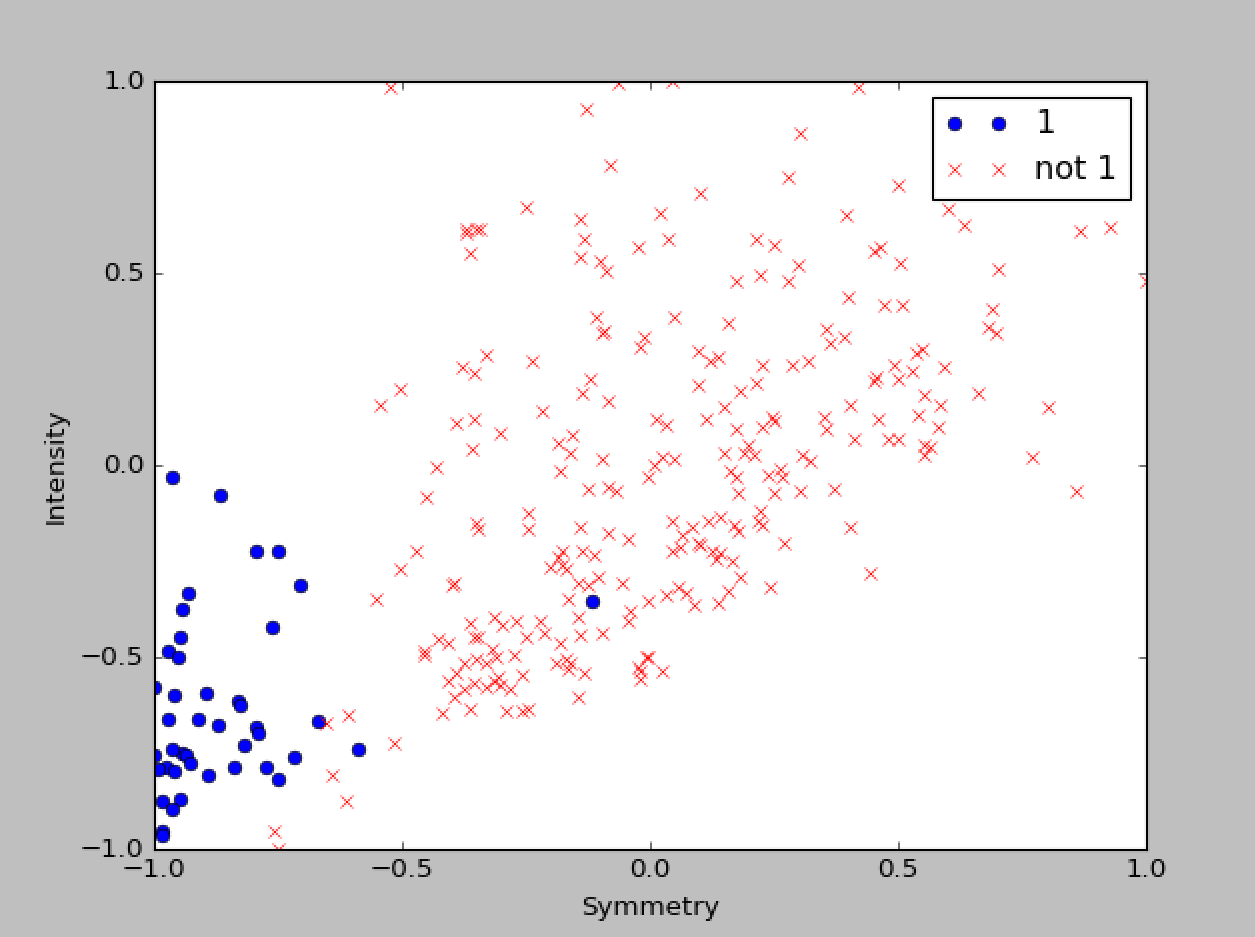
\includegraphics[scale=.5]{2-2.png}

This is the original plot of all the data points. It is pretty clear where you can draw a line in order to have a pretty decent $E_{in}$. It's not linearly separable data, but you can't always have that in the real world.

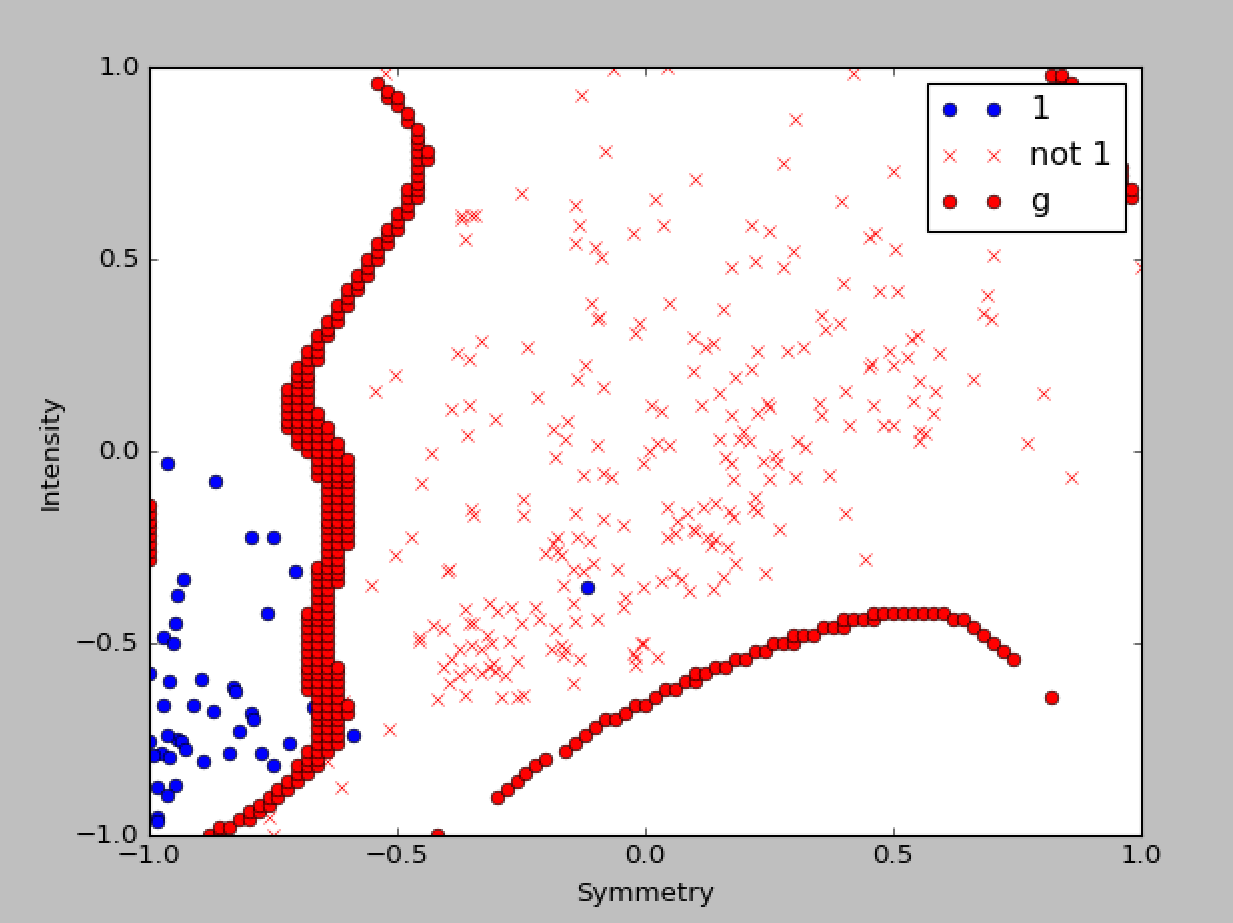
\includegraphics[scale=.5]{2-1.png}

This is the plot with the model without any regularization. As you can see, there is quite a bit of overfitting here. In order to conform with the shape of the 1s, the algorithm outputs a bound that flows with the data points a little bit too much for our comfort. The red dots represent the outputted hypothesis. Also note the large curve on the bottom that's only possible due to a gap in the "not 1" points. We would probably not expect points in this region to actually be considered 1s in real life.

\section*{3. Regularization}
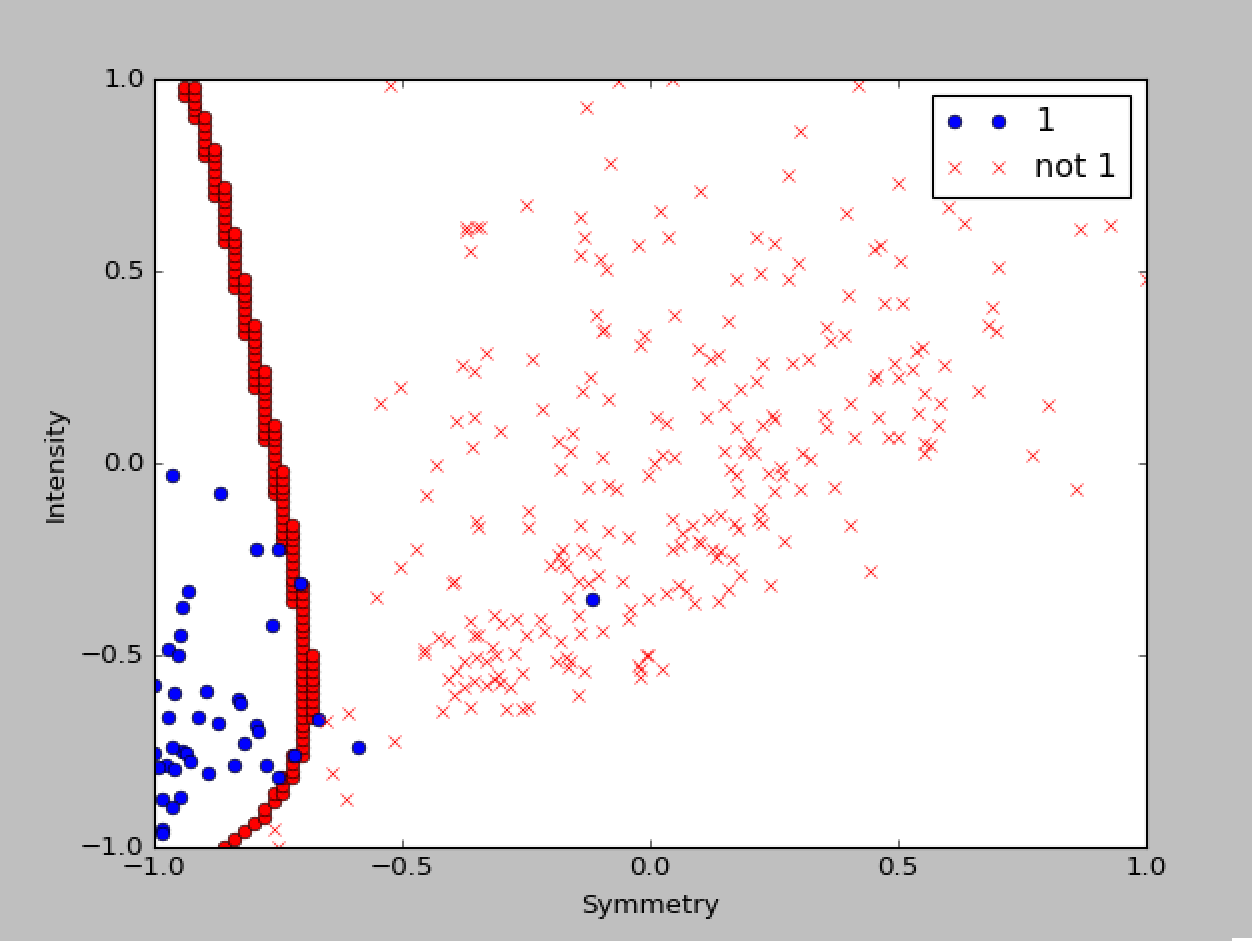
\includegraphics[scale=.5]{3-1.png}

There is a tinge of underfitting here. Notice the blue points that are to the right of the red curve that could be added to the left side of the curve without any loss in $E_{in}$. This is typically a sign that we're probably doing a little too much regularization.

\end{document}